\section{问题一的模型建立与求解}

\subsection{数据预处理与单位统一}

附件 1 给出某天的电价、小区负载功率与光伏发电预测功率，共 144 个 10 分钟时段。负荷与光伏以功率（kW）记录，而储能容量与购电量以电量（kWh）计量，建模前须统一量纲。对任一时段，若平均功率为 $x$ kW，则该时段电量为

\begin{equation}
  E = x\,\Delta t, \qquad \Delta t = \frac{10}{60} = \frac{1}{6}\ \mathrm{h}.
  \label{eq:unit}
\end{equation}

式中：$x$ 为该时段的平均功率（kW）；$E$ 为该时段的电量（kWh）。

据此，小区负荷电量记为 $L(t)$、可利用光伏电量记为 $P(t)$，电价 $\lambda(t)$ 保持元/kWh 不变。储能设备单时段最大充放电电量为

\begin{equation}
  E_{\max} = 5000 \times \frac{1}{6} = 833.33\ \mathrm{kWh},
  \label{eq:emax}
\end{equation}

式中：5000 kW 为储能设备的最大充放电功率；$E_{\max}$ 为单个 10 分钟时段的最大充电量或放电量。按假设 2，附件 1 的 144 行与结果模板的 144 个时段按先后顺序一一对应。

\subsection{无储能基准方案}

为量化储能设备的经济价值，先给出不配置储能设备的基准方案。该方案在任一时段优先使用光伏满足负荷，光伏不足时从外部电网购电，光伏富余时弃光：

\begin{equation}
  G(t) = \max\{L(t)-P(t),\ 0\}, \qquad W(t) = \max\{P(t)-L(t),\ 0\},
  \label{eq:nostorage}
\end{equation}

式中：$G(t)$ 为购电量；$W(t)$ 为弃光量。该基准方案的全天购电费用为 48052.05 元，购电量 61789.94 kWh，弃光量 6247.96 kWh。

\subsection{连续线性规划模型}

以 144 个时段为单位，引入非负决策变量：购电量 $G(t)$、充电量 $C(t)$、放电量 $D(t)$、时段末储电量 $B(t)$ 与弃光量 $W(t)$。优化目标为全天购电费用最小：

\begin{equation}
  \min\ Z_1 = \sum_{t=1}^{144} \lambda(t)\,G(t).
  \label{eq:q1_obj}
\end{equation}

式中：$Z_1$ 为全天购电费用（元）。

约束条件如下。

（1）电力平衡约束。任一时段内，外网购电量、光伏发电量与储能放电量之和，等于负荷电量、储能充电量与弃光量之和：

\begin{equation}
  G(t) + P(t) + D(t) = L(t) + C(t) + W(t), \qquad t = 1,2,\dots,144.
  \label{eq:q1_balance}
\end{equation}

（2）储能状态递推约束。考虑充放电效率后，时段末储电量为

\begin{equation}
  B(t) = B(t-1) + \eta_C\,C(t) - \frac{D(t)}{\eta_D}, \qquad B(0) = 6000,
  \label{eq:q1_soc}
\end{equation}

式中：$B(0)$ 为当天 0:00 的储电量，取 6000 kWh。

（3）储电量上下限约束。为避免过度充电或放电，

\begin{equation}
  1200 \le B(t) \le 10800, \qquad t = 1,2,\dots,144,
  \label{eq:q1_socbound}
\end{equation}

式中：1200 kWh 与 10800 kWh 分别为储能设备允许运行的下限与上限。

（4）充放电功率约束与弃光、非负约束：

\begin{equation}
  0 \le C(t) \le E_{\max}, \qquad 0 \le D(t) \le E_{\max}, \qquad 0 \le W(t) \le P(t).
  \label{eq:q1_power}
\end{equation}

（5）日初日末储电量相等约束。题目要求储能设备在 0:00 与 24:00 的储电量相同：

\begin{equation}
  B(144) = B(0) = 6000.
  \label{eq:q1_terminal}
\end{equation}

式~\eqref{eq:q1_obj} 至式~\eqref{eq:q1_terminal} 构成一个连续线性规划模型，其决策变量与约束个数均为百级规模，可由单纯形法类算法求得全局最优解\cite{ref1,ref2}。

\subsection{显式充放电互斥的混合整数线性规划模型}

连续线性规划中，充电量 $C(t)$ 与放电量 $D(t)$ 各自独立受上界约束，理论上允许出现同一时段既充电又放电的解。为从结构上消除该可能性，引入 0--1 状态变量 $z(t)$ 并追加互斥约束：

\begin{equation}
  0 \le C(t) \le E_{\max}\,z(t), \qquad 0 \le D(t) \le E_{\max}\,[1-z(t)], \qquad z(t)\in\{0,1\},
  \label{eq:q1_mutex}
\end{equation}

式中：$z(t)$ 为时段 $t$ 的充放电状态变量，$z(t)=1$ 时允许充电、放电量被强制为零，$z(t)=0$ 时允许放电、充电量被强制为零。目标函数与其余约束与上一小节完全相同，模型由连续线性规划转化为混合整数线性规划。

\subsection{求解结果与分析}

上述模型由 Python 的 SciPy 调用 HiGHS 求解器求解。连续线性规划与混合整数线性规划的整数相对间隙均为 0，两条思路都取得全天购电费用的全局最优解 35126.95 元。按照题目表 1、表 2 的字段与指定时段，混合整数规划的购电与储能结果分别列于表 2、表 3；三种方案的全年对比见表 4，调度结果对比如图~\ref{fig:q1_compare} 所示。

\threelinetable{表 2\quad 问题一指定时段的购电结果（按题目表 1 格式）}{l r l r l r}{%
  \textbf{时间段} & \textbf{购电量/kWh} & \textbf{时间段} & \textbf{购电量/kWh} & \textbf{时间段} & \textbf{购电量/kWh}%
}{%
  10:00--10:10 & 0.00 & 12:00--12:10 & 486.40 & 14:00--14:10 & 0.00 \\
  16:00--16:10 & 394.93 & 18:00--18:10 & 636.98 & 20:00--20:10 & 0.00 \\
  \multicolumn{2}{c}{全天购电量/kWh} & 59482.70 & \multicolumn{2}{c}{全天购电费/元} & 35126.95
}

\threelinetable{表 3\quad 问题一指定时段的储能结果（按题目表 2 格式）}{l r r l r r}{%
  \textbf{时间段} & \textbf{充电量/kWh} & \textbf{放电量/kWh} & \textbf{时间段} & \textbf{充电量/kWh} & \textbf{放电量/kWh}%
}{%
  0:00--4:00 & 4500.00 & 0.00 & 4:00--8:00 & 833.33 & 6365.84 \\
  8:00--12:00 & 4787.96 & 1703.00 & 12:00--16:00 & 5286.04 & 91.10 \\
  16:00--20:00 & 0.00 & 5780.13 & 20:00--24:00 & 5333.33 & 2859.87 \\
  \multicolumn{2}{c}{0:00 储电量/kWh} & 6000.00 & \multicolumn{2}{c}{24:00 储电量/kWh} & 6000.00
}

\threelinetable{表 4\quad 问题一三种方案的调度结果对比}{l r r r}{%
  \textbf{指标} & \textbf{无储能基准} & \textbf{连续线性规划} & \textbf{混合整数规划}%
}{%
  购电费用/元 & 48052.05 & 35126.95 & 35126.95 \\
  较无储能节省费用/元 & 0.00 & 12925.10 & 12925.10 \\
  较无储能节省率 & 0.00\% & 26.90\% & 26.90\% \\
  全天购电量/kWh & 61789.94 & 59482.70 & 59482.70 \\
  全天充电量/kWh & 0.00 & 20740.67 & 20740.67 \\
  全天放电量/kWh & 0.00 & 16799.94 & 16799.94 \\
  弃光量/kWh & 6247.96 & 0.00 & 0.00 \\
  同时充放电时段数 & 0 & 0 & 0 \\
}

\begin{figure}[H]
  \centering
  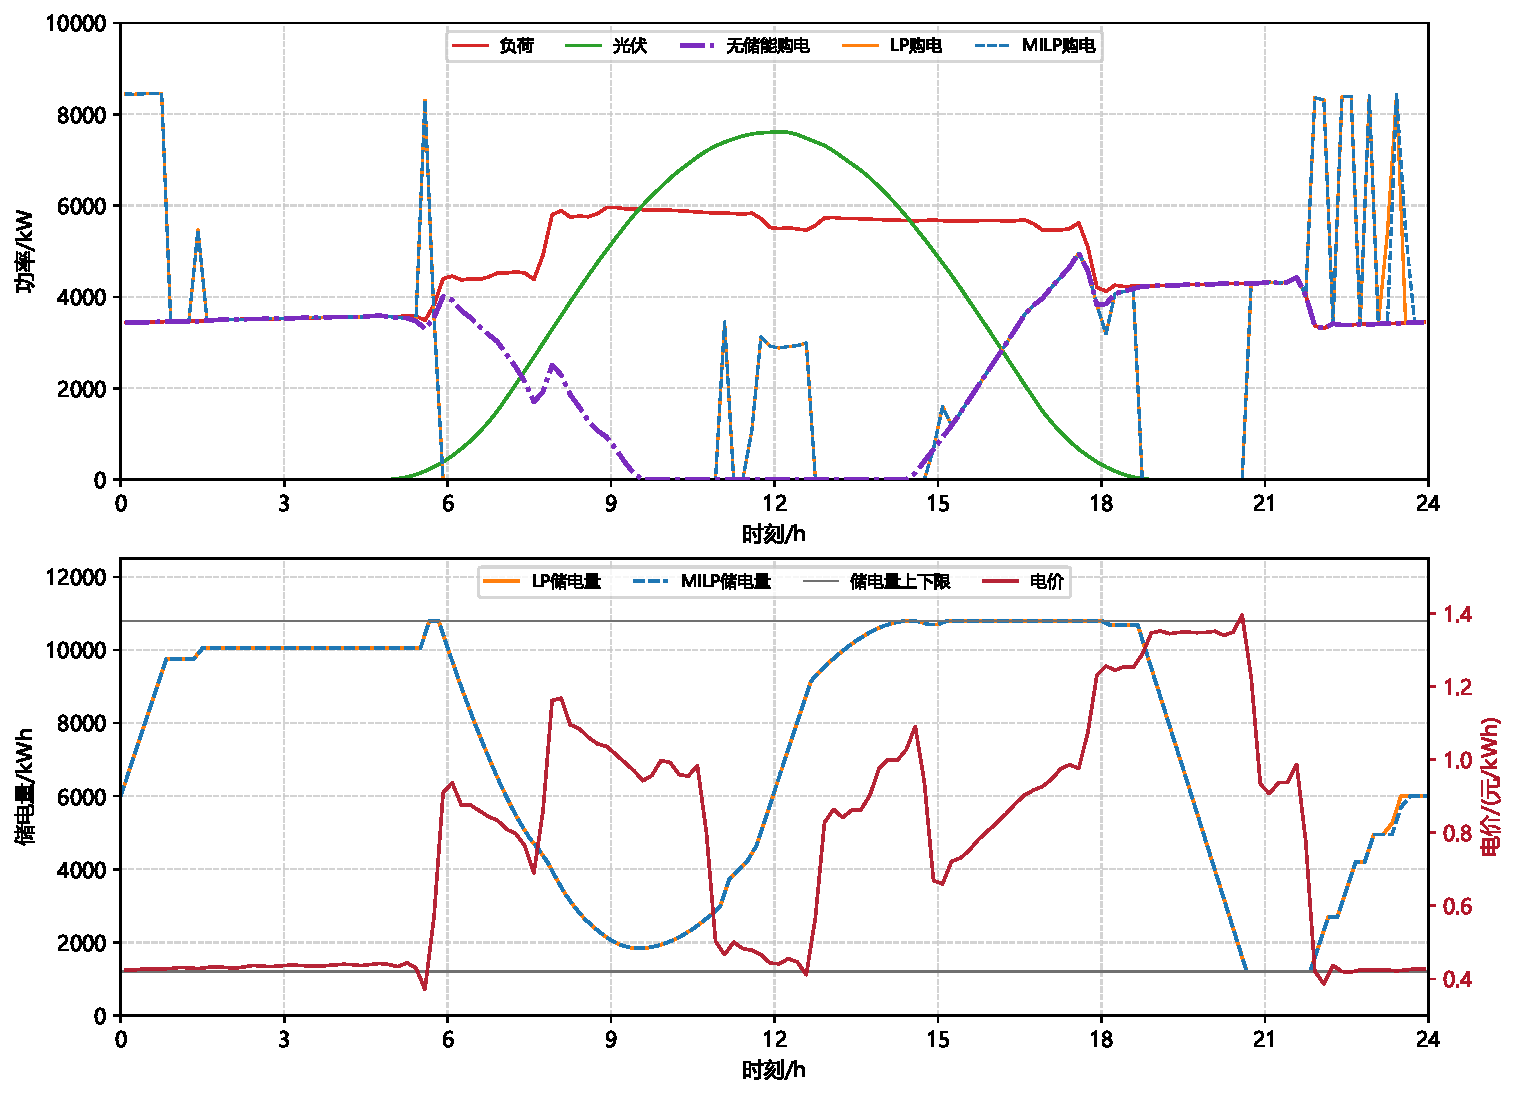
\includegraphics[width=0.72\textwidth]{../figures/问题一/问题一_三种方案调度结果对比.pdf}
  \caption{问题一三种方案的调度结果对比}
  \label{fig:q1_compare}
\end{figure}

由表 4 可见，配置储能设备后全天购电费用下降 26.90\%，弃光量由 6247.96 kWh 降为 0，全天购电量也略有减少。储能设备一方面通过峰谷电价套利降低了高价时段的购电量，另一方面吸收了午间富余的光伏电量，两方面收益共同覆盖了充放电过程中的效率损失。

连续线性规划与混合整数规划的最优费用与全天汇总量完全一致，说明连续松弛在本数据下已经给出了满足充放电互斥条件的最优方案，显式加入 0--1 变量并未改变最优值，只提供了结构上的互斥保证。两种方案在 23:10--23:20 与 23:30--23:40 两个时段的轨迹略有差异，但两时段电价相同，充电量可在其间等价移动，属于多重最优解导致的等价调度方案。
